% ЕМТ 2024, VI клас — точен LaTeX препис от официалните файлове в Klasirane.com.
% Условия: https://klasirane.com/api/competitions/EMT/All/2024/6%20%D0%BA%D0%BB/probs
% SHA-256 (условия): 3c2cc4d07a59f96024e853a7f7e454c35672530043d1fa2d90c90a85ccecfc92
% Решения: https://klasirane.com/api/competitions/EMT/All/2024/6%20%D0%BA%D0%BB/sol
% SHA-256 (решения): 312eb239f682013666a453b76df832d2855229aed94051dba91dd28397d20ab6
% Точковите оценки, правописът, формулировките и видимите печатни грешки са запазени от източника.
% Файлът с условията е сканирано изображение; видимите страници са проверени пряко.
% JPEG фигурите са извлечени без промяна от официалния PDF с решенията; табличните фигури са растеризирани без редакция от векторното PDF съдържание.

Задача 6.1. В аквариум с форма на правоъгълен паралелепипед имало определено количество вода. При почистване източили 40\% от водата. След това добавили филтрирана вода, при което увеличили с 40\% количеството вода, останало след източването. Накрая в аквариума имало 2,1 литра вода.

а) Колко литра вода имало в аквариума отначало?

б) Широчината на дъното на аквариума е 20 cm и е с 20\% по-малка от неговата дължина. Околната повърхнина на аквариума е 7,2 dm$^2$. Колко процента от обема на аквариума са били запълнени с вода отначало?

Решение. а) Нека отначало в аквариума е имало $x$ литра вода. След източването са останали $60\%x$ литра, а след доливането на филтрираната вода, в аквариума имало $140\%\cdot60\%x=84\%x$ литра вода. От равенството $84\%x=2,1$ намираме $x=2,5$ литра.

б) Широчината на дъното $a=20$ cm е с 20\% по-малка от дължината $b$, т.е. е равна на $80\%b$. От равенството $20=80\%b$ намираме $b=25$ cm. Обиколката на дъното е $P=90$ cm и тъй като $S=7,2$ dm$^2=720$ cm$^2$, височината на аквариума е $c=S:P=720:90=8$ cm.

Обемът на аквариума е $V=20\cdot25\cdot8=4000$ cm$^3=4$ dm$^3$.

Водата отначало е $\dfrac{2,5}{4}=62,5\%$ от обема на аквариума.

Оценяване. а) Пълно решение: 3 точки.

Намиране, че крайното количество е 84\% от първоначалното – 2 точки.

Определяне на началното количество вода – 1 точка.

Ако се решава като рачешка задача, по 1,5 т. за всяка стъпка.

б) Пълно решение: 3 точки.

Намиране на дължината – 1 точка.

Намиране на виочината – 1 точка.

Намиране на обема и определяне на търсения процент – 1 точка.

Задача 6.2. За дадени числа $a,b,c,d$ означаваме
$$
\begin{vmatrix}a&b\\c&d\end{vmatrix}=a\cdot d-b\cdot c.
$$
Например,
$$
\begin{vmatrix}1&-2\\3&-4\end{vmatrix}=1\cdot(-4)-(-2)\cdot3=2.
$$

а) Пресметнете сбора
$$
S=\begin{vmatrix}0&-1\\-3&2\end{vmatrix}+\begin{vmatrix}1&-2\\-4&3\end{vmatrix}+\begin{vmatrix}2&-3\\-5&4\end{vmatrix}+\cdots+\begin{vmatrix}43&-44\\-46&45\end{vmatrix}.
$$

б) Намерете числото $X$ в равенството
$$
\begin{vmatrix}X&\frac12\\\frac13&-1\end{vmatrix}+\begin{vmatrix}X&\frac13\\\frac14&2\end{vmatrix}+\begin{vmatrix}X&\frac14\\\frac15&-3\end{vmatrix}+\begin{vmatrix}X&\frac15\\\frac16&4\end{vmatrix}+\cdots+\begin{vmatrix}X&\frac1{23}\\\frac1{24}&22\end{vmatrix}=\frac{11}{12}.
$$

Решение. а) Забелязваме, че
$$
\begin{vmatrix}a&-b\\-c&d\end{vmatrix}=a\cdot d-(-b)\cdot(-c)=a\cdot d-b\cdot c=\begin{vmatrix}a&b\\c&d\end{vmatrix}.
$$
Следователно
$$
S=\begin{vmatrix}0&1\\3&2\end{vmatrix}+\begin{vmatrix}1&2\\4&3\end{vmatrix}+\begin{vmatrix}2&3\\5&4\end{vmatrix}+\cdots+\begin{vmatrix}43&44\\46&45\end{vmatrix}=
$$
$$
=(0\cdot2-1\cdot3)+(1\cdot3-2\cdot4)+(2\cdot4-3\cdot5)+\cdots+(43\cdot45-44\cdot46)=0-44\cdot46=-2024,
$$
тъй като в получения сбор събираемите, без първото и последното, се разделят на двойки противоположни със сбор 0.

б) Даденото равенство се записва във вида
$$
-X-\frac12\cdot\frac13+2X-\frac13\cdot\frac14-3X-\frac14\cdot\frac15+4X-\frac15\cdot\frac16+\cdots+22X-\frac1{23}\cdot\frac1{24}=\frac{11}{12}.
$$
Имаме
$$
-X+2X-3X+4X+\cdots+22X=(-1+2-3+4-5+\cdots-21+22)X=11X,
$$
тъй като $-1+2=-3+4=\cdots=-21+22=1$. От друга страна,
$$
-\frac12\cdot\frac13-\frac13\cdot\frac14-\cdots-\frac1{23}\cdot\frac1{24}=-\left(\frac12-\frac13+\frac13-\frac14+\cdots+\frac1{23}-\frac1{24}\right)=
$$
$$
=-\left(\frac12-\frac1{24}\right)=-\frac{11}{24}.
$$
Получаваме $11X-\dfrac{11}{24}=\dfrac{11}{12}$, откъдето намираме $X=\dfrac18$.

Оценяване. а) Пълно решение: 2 точки.

б) Пълно решение: 4 точки.

Определяне на коефициента пред $X$ – 1,5 точки.

Пресмятане на телескопичния сбор – 1,5 точки.

Намиране на $X$ – 1 точка.

Задача 6.3. Даден е триъгълник $ABC$. На страната $AB$ е отбелязана точка $M$ така, че $AM=\dfrac12AB$; на страната $AC$ е отбелязана точка $K$ така, че $AK=\dfrac13AC$; на страната $BC$ е отбелязана точка $L$ така, че $BL=\dfrac14BC$. Отсечките $KL$ и $CM$ се пресичат в точка $O$ и лицето на четириъгълника $AMOK$ е 36 cm$^2$.

Намерете лицето на триъгълника $COL$ и лицето на триъгълника $ABC$.

Решение. Ако $h_L$ е разстоянието от $L$ до $AC$, а $h_A$ е разстоянието от $A$ до $BC$, имаме
$$
\frac{S_{CKL}}{S_{ALC}}=\frac{\frac12\cdot CK\cdot h_L}{\frac12\cdot AC\cdot h_L}=\frac{CK}{AC}=\frac23,
\qquad
\frac{S_{ALC}}{S_{ABC}}=\frac{\frac12\cdot CL\cdot h_A}{\frac12\cdot BC\cdot h_A}=\frac{CL}{BC}=\frac34
$$
и като умножим тези равенства, получаваме
$$
\frac{S_{CKL}}{S_{ABC}}=\frac23\cdot\frac34=\frac12.
$$

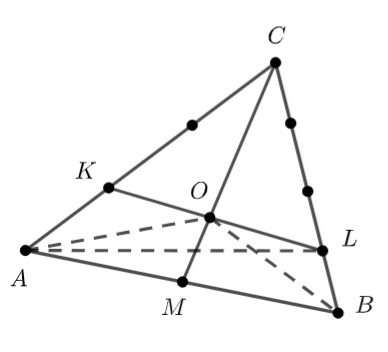
\includegraphics[max width=0.42\textwidth, alt={Триъгълник ABC с точките K, L, M и пресечната точка O}, center]{assets/6-3-geometry.jpeg}

Следователно лицето на триъгълника $CKL$ е равно на половината от лицето на триъгълника $ABC$. От друга страна,
$$
\frac{S_{AMC}}{S_{ABC}}=\frac{\frac12\cdot AM\cdot h_C}{\frac12\cdot AB\cdot h_C}=\frac{AM}{AB}=\frac12,
$$
т.е. лицето на триъгълника $AMC$ е равно на половината от лицето на триъгълника $ABC$ (по-нататък ще използваме това свойство на медианата без доказателство).

Следователно $S_{AMC}=S_{CKL}$, т.е.
$$
S_{AMOK}+S_{KOC}=S_{KOC}+S_{COL}\Longleftrightarrow S_{AMOK}=S_{COL}.
$$
Така получихме, че $S_{COL}=36$ cm$^2$.

От $\dfrac{S_{COB}}{S_{COL}}=\dfrac{BC}{LC}=\dfrac43$ следва, че
$$
S_{COB}=\frac43S_{COL}=48\text{ cm}^2.
$$
Тъй като $CM$ е медиана в триъгълника $ABC$, то $S_{AMC}=S_{BMC}$. Освен това, $OM$ е медиана в триъгълника $ABO$ и $S_{AMO}=S_{BMO}$. Като извадим почленно двете равенства. получаваме
$$
S_{AOC}=S_{COB},\text{ т.е. }S_{AOC}=48\text{ cm}^2.
$$
Но $\dfrac{S_{AOK}}{S_{AOC}}=\dfrac{AK}{AC}=\dfrac13$, следователно
$$
S_{AOK}=\frac13S_{AOK}=16\text{ cm}^2.
$$
Тогава
$$
S_{AOM}=S_{AMOK}-S_{AOK}=36-16=20\text{ cm}^2,
$$
откъдето и $S_{BMO}=20$ cm$^2$. Така $S_{ABC}=2\cdot(20+48)=136$ cm$^2$.

Оценяване. Доказателство, че лицето на триъгълника $CKL$ е равно на половината от лицето на триъгълника $ABC$ – 2 точки.

Доказателство, че $S_{AMC}=S_{CKL}$ – 1 точка.

Намиране на лицето на $COL$ – 1 точка.

Намиране на $S_{COB}$ – 1 точка.

Намиране на $S_{AOK}$ – 1 точка,

Намиране на $S_{ABC}$ – 1 точка.

Задача 6.4. Серпентина ще наричаме квадратна таблица $n\times n$, в която са записани последователни цели числа по следния начин: най-малкото от числата е в горния ляв ъгъл; в първия ред числата нарастват отляво надясно; в последното поле от реда се прави завой към полето под него; във втория ред числата нарастват отдясно наляво и т.н. (Стрелките на фиг. 1 показват реда на попълване на последователните числа в серпентина $3\times3$.)

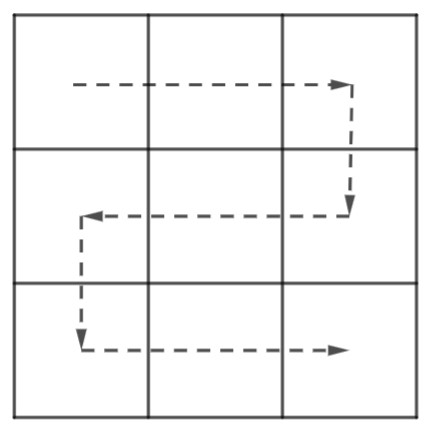
\includegraphics[max width=0.28\textwidth, alt={Ред на попълване на серпентина три по три}, center]{assets/6-4-serpentine-path.jpeg}

При всеки ход се избират две съседни полета в таблицата (т.е. полета с обща страна) и към числата в тях се прибавя едно и също число. На фиг. 2 са показани два поредни хода в таблица $3\times3$: при първия ход към числата в сивите квадратчета се прибавя 2, а при втория ход към избраните квадратчета се прибавя $(-6)$.

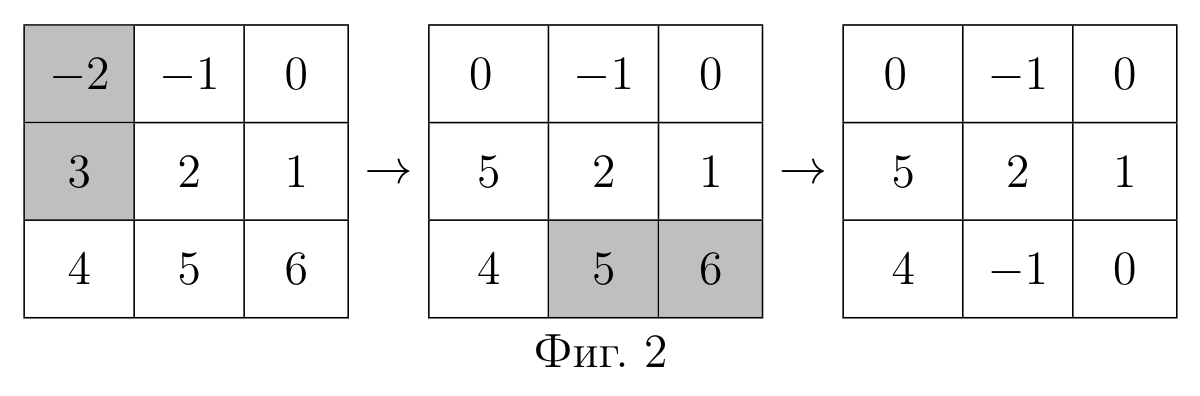
\includegraphics[max width=0.78\textwidth, alt={Два поредни хода в таблица три по три}, center]{assets/6-4-two-moves.png}

Една серпентина наричаме \textbf{особена}, ако след няколко хода от нея може да се получи таблица, във всички полета на която е записана 0.

а) Намерете всички особени серпентини при $n=5$.

б) Съществува ли особена серпентина при $n=10$?

Решение. Ако оцветим таблицата шахматно, при всеки ход едно бяло и едно черно поле се увеличават или намаляват с едно и също число. Това означава, че разликата между сбора на числата в белите полета и сбора на числата в черните полета се запазва.

а) Общият вид на серпентина $5\times5$ е следният:

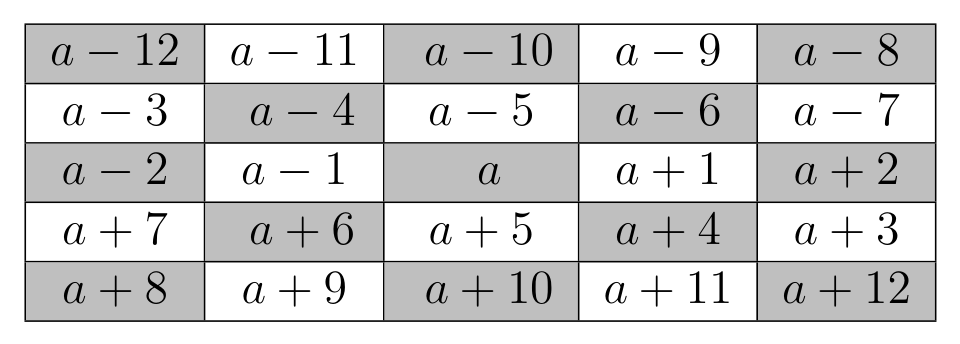
\includegraphics[max width=0.72\textwidth, alt={Общ вид на шахматно оцветена серпентина пет по пет}, center]{assets/6-4-general-5x5.png}

Сборът на числата в черните полета е $S_b=13a$, а сборът на числата в белите полета е $S_w=12a$. След всеки ход се запазва разликата между сбора на числата в черните полета и сбора на числата в белите полета, който отначало е $S_b-S_w=a$.

Следователно ако серпентината $5\times5$ е особена, то $a=0$.

Остава да покажем, че при $a=0$ с няколко хода може да се получи таблица само с 0. В таблицата

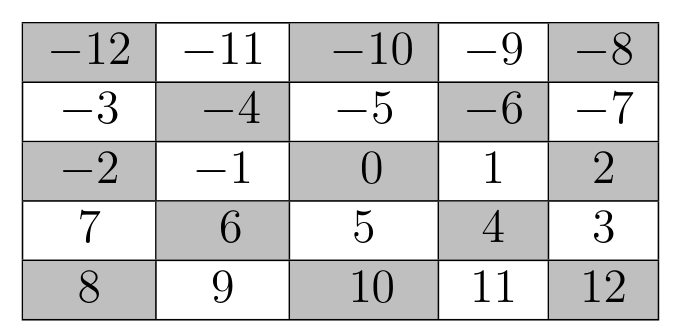
\includegraphics[max width=0.52\textwidth, alt={Шахматно оцветена серпентина пет по пет с централна нула}, center]{assets/6-4-zero-5x5.png}

разделяме полетата по двойки и след 10 хода
$$
(-12;-11)\to(0;1),\ (-10;-9)\to(1;2),\ (-8;-7)\to(2;3),
$$
$$
(-6;-5)\to(3;4),\ (-4;-3)\to(4;5),\ (-2;-1)\to(5;6),
$$
$$
(7;8)\to(0;1),\ (9;10)\to(1;2),\ (5;4)\to(2;1),\ (3;12)\to(2;11)
$$
стигаме до таблица, в която има 11 двойки съседни полета, във всяка от които са записани равни числа:

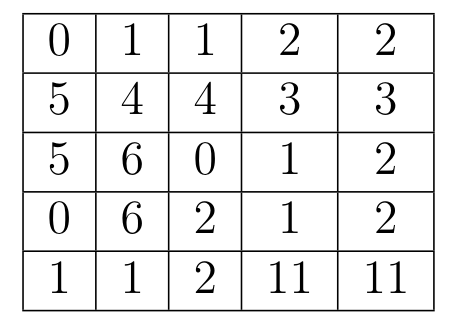
\includegraphics[max width=0.34\textwidth, alt={Таблица пет по пет с единадесет двойки съседни равни числа}, center]{assets/6-4-paired-5x5.png}

От тук с 11 хода получаваме таблица само с 0.

б) В серпентина $10\times10$ са записани 100 числа; ако в горния ляв ъгъл е числото $a-50$, най-голямото число в таблицата $a+49$ ще е записано в долния ляв ъгъл. Сборът на всички числа в таблицата е $100a-50$.

Ако оцветим таблицата шахматно така, че $a-50$ да е в черно поле, сборът на числата в черните полета ще е
$$
S_b=(a-50)+(a-48)+\cdots+(a-2)+a+(a+2)+\cdots+(a+48)=50a-50,
$$
а сборът на числата в белите полета ще е
$$
S_w=(100a-50)-(50a-50)=50a,
$$
което означава, че $S_w-S_b=50$ след всеки ход. Това означава, че не съществува особена серпентина $10\times10$.

Забележка. По същия начин може да се докаже, че особена серпентина съществува само за нечетно $n$.

Оценяване. За шахматно оцветяване и съображението, че сборът на числата в черните полета се променя по същия начин като сбора на числата в белите полета – 1 т.

а) Доказателство, че в централното квадратче е записана 0 – 2 точки.

Пример как се стига до таблица само с 0 – 2 точки.

б) Доказателство, че разликата на сбора на числата в черните полета и сбора на числата в белите полета е ненулева константа – 2 точки.
